When it comes to a program with many conditional statements, usually if() statements, the effectiveness of the branch prediction often determines the overall performance. If the branch is predicted accurately, it has almost no cost. If the branch is mispredicted half the time, it can be as expensive as ten or more regular arithmetic instructions.

It is very important to understand that the hardware branch prediction is based on the conditional instructions executed by the processor. As such, the processor's understanding of what a condition is can be different from our understanding. The following example helps to drive this point home, with force:

\hspace*{\fill} \\ %插入空行
\noindent
\textbf{02\_branch.C}
\begin{lstlisting}[style=styleCXX]
std::vector<unsigned long> v1(N), v2(N);
std::vector<int> c1(N), c2(N);
for (size_t i = 0; i < N; ++i) {
	v1[i] = rand();
	v2[i] = rand();
	c1[i] = rand() & 0x1;
	c2[i] = !c1[i];
}
unsigned long* p1 = v1.data();
unsigned long* p2 = v2.data();
int* b1 = c1.data();
int* b2 = c2.data();
for (auto _ : state) {
	unsigned long a1 = 0, a2 = 0;
	for (size_t i = 0; i < N; ++i) {
		if (b1[i] || b2[i]) { // !!!
			a1 += p1[i];
		} else {
			a1 *= p2[i];
		}
	}
	benchmark::DoNotOptimize(a1);
	benchmark::DoNotOptimize(a2);
	benchmark::ClobberMemory();
}
\end{lstlisting}

Of interest here is the condition if (b1[i] || b2[i]): by construction, it always evaluates to true, so we can expect the perfect prediction rate from the processor. Of course, I would not be showing this example to you if it was as simple as that. What is, logically, a single condition to us is, to the CPU, two separate conditional branches: half the time, the overall result is true because of the first branch, and the other half the time, it is the second branch that makes it true. The overall result is always true, but it is impossible to predict which of the branches makes it so. The result is quite unfortunate:

\hspace*{\fill} \\ %插入空行
\begin{center}
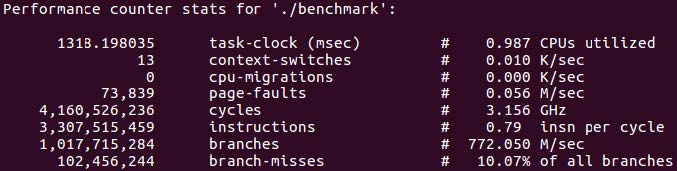
\includegraphics[width=0.9\textwidth]{content/1/chapter3/images/27.jpg}\\
Figure 3.27 – Branch prediction profile of a "fake" branch
\end{center}

The profiler shows the branch prediction rate that is just as poor as that of a truly random branch. The performance benchmark confirms our expectations:


\hspace*{\fill} \\ %插入空行
\begin{center}
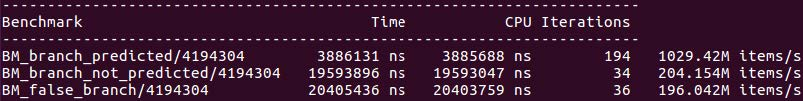
\includegraphics[width=0.9\textwidth]{content/1/chapter3/images/28.jpg}\\
Figure 3.28
\end{center}

The performance of the fake branch (that isn't really a branch at all) is just as bad as that of a truly random, unpredictable branch, and is far worse than that of a well-predicted branch.

In a real program, you should not encounter such unnecessary conditional statements. What is very common, however, is a complex conditional expression that almost always evaluates to the same value but for different reasons. For example, we may have a condition that is very rarely false:

\begin{lstlisting}[style=styleCXX]
if ((c1 && c2) || c3) {
	… true branch …
} else {
	… false branch …
}
\end{lstlisting}

However, nearly half the time, c3 is true. When c3 is false, c1 and c2 are usually both true. The overall condition should be easily predictable, and the true branch is taken. However, from the processor's point of view, it is not a single condition but three separate conditional jumps: if c1 is true, then c2 must be checked. If c2 is also true, then the execution jumps to the first instruction of the true branch. If one of c1 or c2 is false, then c3 is checked, and, if it's true, the execution again jumps to the true branch.

The reason this evaluation must be done step by step and in that specific order is that the C++ standard (and the C standard before it) dictates that the logical operations such as \&\& and || are short-circuited: as soon as the result of the entire expression is known, the evaluation of the rest of the expression should stop. This is particularly important when the conditions have side effects:

\begin{lstlisting}[style=styleCXX]
if (f1() || f2()) {
	… true branch …
} else {
	… false branch …
}
\end{lstlisting}

Now the function f2() will be called only if f1() returns false. In the previous example, the conditions were simply boolean variables c1, c2, and c3. The compiler could have detected that there are no side effects and that evaluating the entire expression to the end will not change the observable behavior. Some compilers do this optimization; if our fake branch benchmark were compiled with such a compiler, it would have shown the performance of a well-predicted branch. Most compilers, unfortunately, do not recognize this as a potential problem (and, in fact, there is no way for the compiler to know that the entire expression usually evaluates to true, even if its parts do not). So, this is an optimization that the programmer must usually do manually.

Assume that the programmer knows that one of the two branches of the if() statement is taken much more often. For example, the else branch could correspond to an error situation or some other exceptional condition that must be handled properly but should not arise under normal operation. Let us also assume that we did things right and verified, using the profiler, that the individual conditional instructions that make up the complex boolean expression are not well-predicted. How do we optimize the code?

The first impulse may be to move the condition evaluation out of the if() statement:

\begin{lstlisting}[style=styleCXX]
const bool c = c1 && c2) || c3;
if (c) { … } else { … }
\end{lstlisting}

However, this is almost guaranteed not to work, for two reasons. First, the condition expression is still using the logical \&\& and || operations, so the evaluation still must be short-circuited and will require separate and unpredictable branches. Second, the compiler will likely optimize this code by removing the unnecessary temporary variable c, so the resulting object code probably will not change at all.

In the case of a loop over an array of conditional variables, a similar transformation may be effective. For example, this code is likely to suffer from poor branch prediction:

\begin{lstlisting}[style=styleCXX]
for (size_i i = 0; i < N; ++i) {
	if ((c1[i] && c2[i]) || c3[i]) { … } else { … }
}
\end{lstlisting}

However, if we pre-evaluate all the conditional expressions and store them in a new array, most compilers will not eliminate that temporary array:

\begin{lstlisting}[style=styleCXX]
for (size_i i = 0; i < N; ++i) {
	c[i] = (c1[i] && c2[i]) || c3[i];
}
…
for (size_i i = 0; i < N; ++i) {
	if (c[i]) { … } else { … }
}
\end{lstlisting}

Of course, the boolean expression used to initialize c[i] now suffers from branch misprediction, so this transformation works only if the second loop is executed many more times than the initialization loop.

Another optimization that is usually effective is to replace the logical \&\& and || operations with addition and multiplication or with bitwise \& and | operations. Before doing this, you must be certain that the arguments to the \&\& and || operations are booleans (have values of zero or one) and not integers: even though a value of, say, 2 is interpreted as true, the result of the expression 2 \& 1 is not the same as the result of bool(2) \& bool(1). The former evaluates to 0 (false) while the latter gives us the expected and correct answer, 1 (or true).

We can compare the performance of all these optimizations in a benchmark:

\hspace*{\fill} \\ %插入空行
\begin{center}
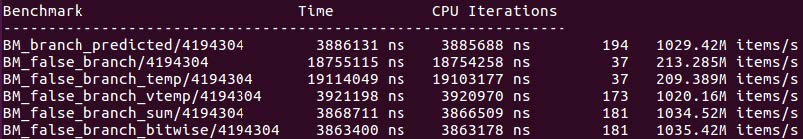
\includegraphics[width=0.9\textwidth]{content/1/chapter3/images/29.jpg}\\
Figure 3.29
\end{center}

As you can see, the naïve attempt to optimize the false branch by introducing a temporary variable, BM\_false\_branch\_temp, was utterly ineffective. Using a temporary vector gives us the expected performance of a perfectly predicted branch because all elements of the temporary vector are equal to true, and that is what the branch predictor learns (BM\_false\_branch\_vtemp). Replacing the logical || with either arithmetic addition (+) or the bitwise | produces similar results.

You should keep in mind that the last two transformations, using arithmetic or bitwise operations instead of logic operations, change the meaning of your code: specifically, all arguments to the operations in the expression are always evaluated, including their side effects. It is up to you to decide whether this change will affect the correctness of your program. If these side effects are also expensive, then the overall performance change may end up being not in your favor. For example, if evaluating f1() and f2() is very timeconsuming, replacing the logical || in the expression f1() || f2() by the equivalent arithmetic addition (f1() + f2()) may degrade the performance even as it improves the branch prediction.

Overall, there is no standard approach to optimizing the branch prediction in false branches, which is why it is so hard for the compiler to do any effective optimizations as well. The programmer must use problem-specific knowledge, such as whether a particular condition is likely to occur, and combine it with profiling measurements to arrive at the optimal solution.

In this chapter, we have learned how CPU operations affect performance, then progressed to a concrete and practically relevant example of applying this knowledge to code optimization. Before the end, we will learn about one more such optimization.



























